% FYP Defense Presentation
% Beamer slides for thesis: Deploying an Autonomous Indoor Robot with Laser Mapping and Multi-Hop Networking for Disaster Site Exploration

\documentclass[aspectratio=169]{beamer}
\usetheme{Madrid}
\usecolortheme{default}
\setbeamertemplate{navigation symbols}{}
\setbeamertemplate{footline}{}

\title{Deploying an Autonomous Indoor Robot with Laser Mapping and Multi-Hop Networking for Disaster Site Exploration}
\author{
  Habeel Ali (FA22-BCE-067) \\
  Tahreem Shahid (FA22-BCE-035) \\
  Ramisha Ikram (FA22-BCE-024) \\
  Ibrahim Imran (FA22-BCE-032)
}
\date{\today}
\institute{FYP Defense}

\usepackage{graphicx}
\usepackage{booktabs}

\begin{document}

\begin{frame}
\titlepage
\end{frame}

\begin{frame}{Outline}
\begin{itemize}
\item Problem \& objectives
\item Methodology (SLAM, communication, perception)
\item Implementation (platform \& stack)
\item Results (mapping, communication, perception)
\item Conclusions \& future work
\end{itemize}
\end{frame}

% --- Problem & motivation ---
\begin{frame}{Problem \& Motivation}
\begin{itemize}
\item Disaster response: minimise human risk and cognitive load
\item Need: mapping, hazard detection, visual data collection, resilient communication
\item Indoor, GNSS-denied environments; LiDAR effective without sunlight
\item Challenges: real-time SLAM on embedded hardware, multi-tier connectivity, AI perception with limited onboard power
\end{itemize}
\end{frame}

% --- Objectives ---
\begin{frame}{Objectives}
\begin{enumerate}
\item Implement LiDAR-based SLAM for localisation, mapping, and navigation indoors
\item Formulate mesh-based and hybrid communication with low-bandwidth fallback
\item Integrate AI vision for camera streams, hazard detection, and mission reports
\item Test and integrate the UGV system; measure KPIs
\end{enumerate}
\end{frame}

% --- System overview ---
\begin{frame}{System Overview}
\begin{center}
\includegraphics[width=0.85\textwidth]{figures/system_topology.png}
\end{center}
UGV, multi-tier network (Wi-Fi, 4G, mesh, LoRa), and Ground Control Station (GCS).
\end{frame}

% --- Methodology SLAM & nav ---
\begin{frame}{Methodology: SLAM \& Navigation}
\begin{itemize}
\item \textbf{Cartographer}: 2D SLAM, scan-matching and loop closure (no wheel odometry)
\item \textbf{Nav2}: global (Dijkstra) and local (DWB) planning; costmaps with LiDAR + Kinect
\item \textbf{Frontier-based exploration}: cluster frontiers, score by size, distance, heading; ProxMaP-style U-Net predicts occupancy to prioritise frontiers
\item Map resolution 0.05\,m; 10\,Hz LiDAR
\end{itemize}
\end{frame}

% --- Methodology Communication ---
\begin{frame}{Methodology: Communication}
\begin{itemize}
\item \textbf{Primary}: ESP-WiFi-MESH (deployable nodes along path; added to routing table)
\item \textbf{Fallbacks}: direct Wi-Fi, 4G hotspot, LoRa (SX1278) for telemetry and return-to-base
\item Graceful degradation: video $\rightarrow$ JPEG over mesh $\rightarrow$ telemetry only
\item Nodes: ESP32 DevKit, 2500\,mAh LiPo each
\end{itemize}
\end{frame}

% --- Methodology Perception ---
\begin{frame}{Methodology: Perception}
\begin{itemize}
\item \textbf{YOLOv8}: fire/smoke, extinguisher, human (parallel models)
\item \textbf{LLM} (Llama-4-Scout via Groq): scene description, hazard severity, person re-ID
\item \textbf{X-SDM}: spatial decision memory (revisit vs new location); person profiling for map annotations
\item All inference on GCS (operator GPU); video streamed from UGV
\end{itemize}
\end{frame}

% --- Implementation platform ---
\begin{frame}{Implementation: Platform}
\begin{itemize}
\item \textbf{Compute}: Raspberry Pi~4 (8\,GB), Ubuntu 22.04, ROS~2 Humble
\item \textbf{Sensors}: YDLidar X3 (2D LiDAR, 10\,Hz), Kinect v1 (RGB-D for costmap), USB webcam + ESP32-CAM (720p, 15\,fps)
\item \textbf{Comms}: TP-Link Archer C6 (Wi-Fi AP), ESP32 DevKit mesh nodes, LoRa SX1278
\item \textbf{Power}: 24\,V pack (dual 3s3p 18650); $\sim$2\,h at 0.2\,m/s
\end{itemize}
\end{frame}

% --- UGV front, side, rear ---
\begin{frame}{UGV Platform: Front, Side, Rear}
\begin{columns}[T]
\begin{column}{0.32\textwidth}
\begin{center}
\includegraphics[width=\textwidth]{figures/ugv_front.jpg}\\
\small Front
\end{center}
\end{column}
\begin{column}{0.32\textwidth}
\begin{center}
\includegraphics[width=\textwidth]{figures/ugv_side.jpg}\\
\small Side
\end{center}
\end{column}
\begin{column}{0.32\textwidth}
\begin{center}
\includegraphics[width=\textwidth]{figures/ugv_back.jpg}\\
\small Rear
\end{center}
\end{column}
\end{columns}
\end{frame}

% --- Implementation stack ---
\begin{frame}{Implementation: Software Stack}
\begin{itemize}
\item ROS~2 Humble: Cartographer, Nav2, custom frontier package, TF, rosbridge
\item ProxMaP-style U-Net for map prediction (128$\times$128 crop)
\item GCS: FastAPI backend, WebSocket (rosbridge), web dashboard (map, video, detections, teleop)
\item No onboard GPU; AI on operator workstation
\end{itemize}
\end{frame}

% --- Test environment ---
\begin{frame}{Test Environment}
\begin{columns}
\begin{column}{0.5\textwidth}
\begin{itemize}
\item University department floor
\item $\sim$40\,m $\times$ 30\,m
\item Corridor, lobbies, rooms
\item Operator outside to simulate remote GCS
\end{itemize}
\end{column}
\begin{column}{0.5\textwidth}
\begin{center}
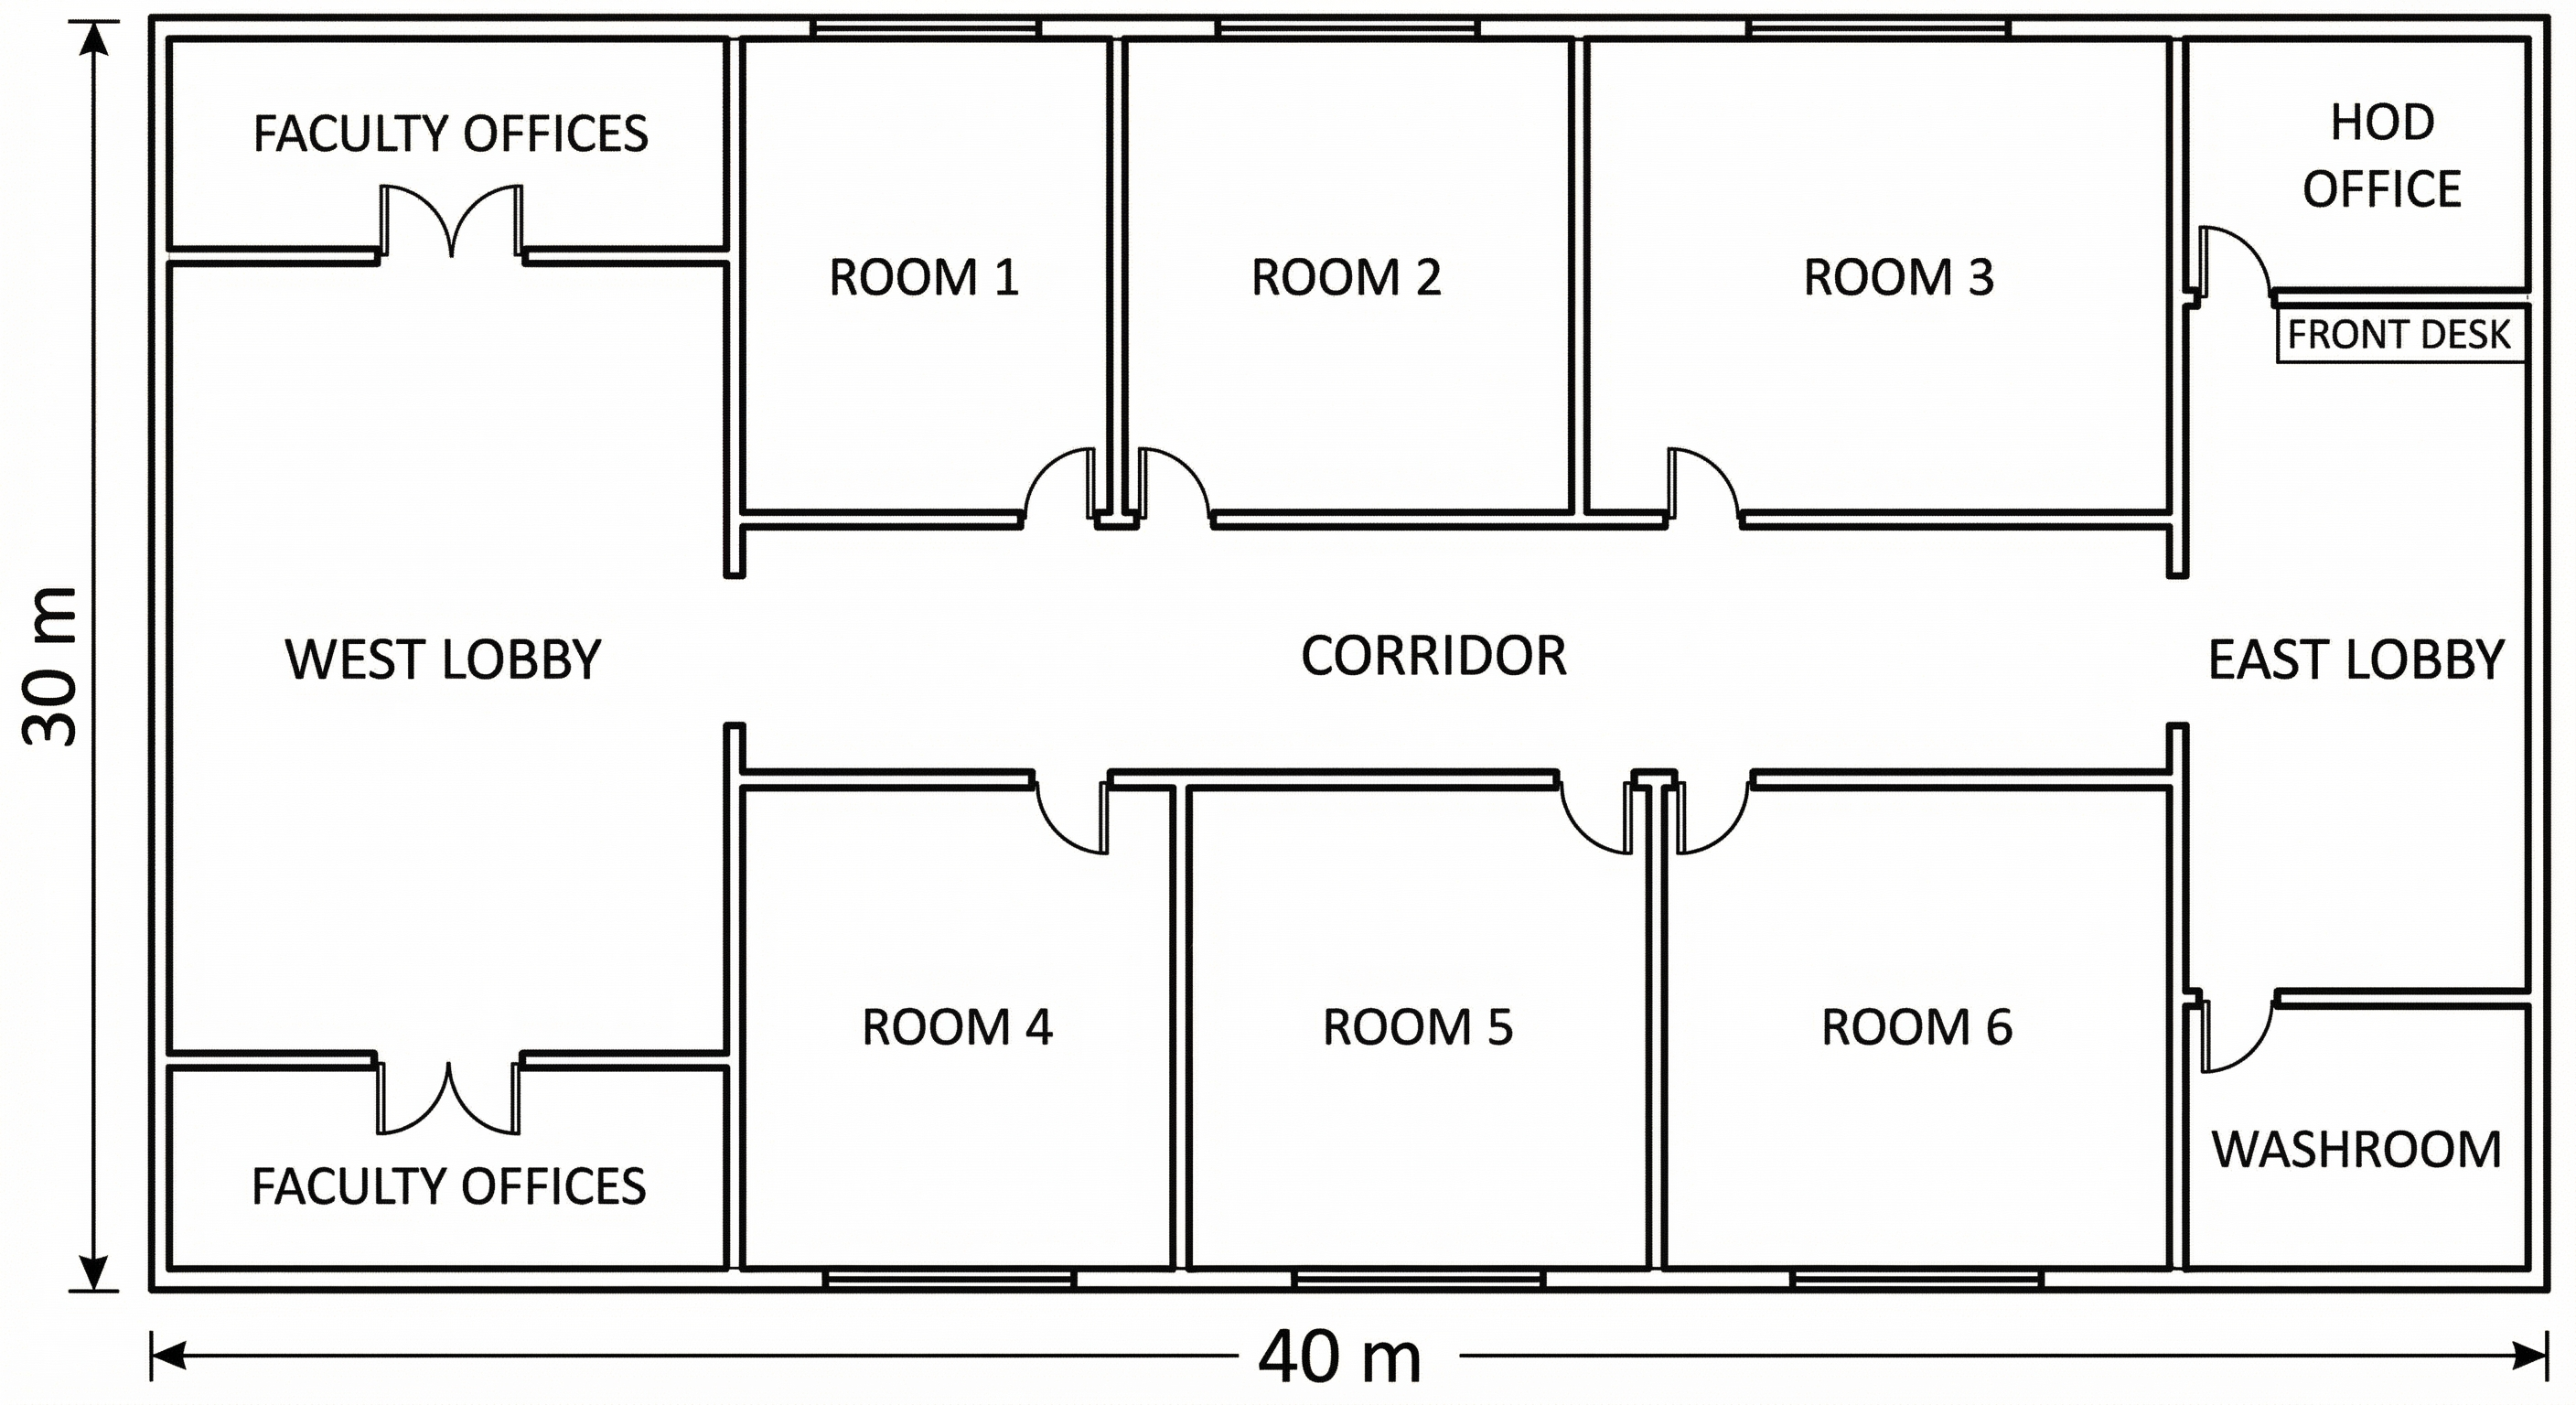
\includegraphics[width=\textwidth]{figures/floor_plan.jpeg}
\end{center}
\end{column}
\end{columns}
\end{frame}

% --- Results mapping ---
\begin{frame}{Results: Mapping \& Exploration}
\begin{itemize}
\item Drift: $<$5\,cm (feature-rich), 20--30\,cm (feature-poor)
\item Map resolution 0.05\,m; CPU 50--60\% (80\% during loop closure)
\item Runtime $\sim$2\,h at 0.2\,m/s
\end{itemize}
\begin{table}
\centering
\small
\begin{tabular}{lcc}
\toprule
\textbf{Metric} & \textbf{Without prediction} & \textbf{With prediction} \\
\midrule
Time to full coverage (min) & 22 & 19 \\
Area at 15\,min (m$^2$) & 260 & 310 \\
Frontier goals reached & 18 & 22 \\
\bottomrule
\end{tabular}
\caption{Frontier scoring: with vs.\ without AI map prediction.}
\end{table}
\end{frame}

% --- Results communication ---
\begin{frame}{Results: Communication}
\begin{table}
\centering
\small
\begin{tabular}{llc}
\toprule
\textbf{Link} & \textbf{Condition} & \textbf{Result} \\
\midrule
Wi-Fi & 25--30\,m LoS & 40--50\,Mbps \\
Wi-Fi & Through rooms & 10--15\,Mbps \\
4G & In coverage & 10--15\,Mbps \\
Mesh (1--2 nodes) & Fallback & 1--2\,Mbps \\
LoRa & Indoors & 50--100\,m \\
\bottomrule
\end{tabular}
\caption{Communication tiers (indoor test environment).}
\end{table}
Multi-tier redundancy: loss of one link does not isolate the robot.
\end{frame}

% --- Results perception ---
\begin{frame}{Results: Perception}
\begin{itemize}
\item YOLOv8 mAP: 70--85\% (disaster-relevant test set)
\item Per-frame inference: 50--100\,ms (GCS GPU)
\item End-to-end: 300--600\,ms (Wi-Fi), 800--1500\,ms (mesh)
\item LLM scene analysis: 200--400\,ms (Groq API)
\end{itemize}
\begin{center}
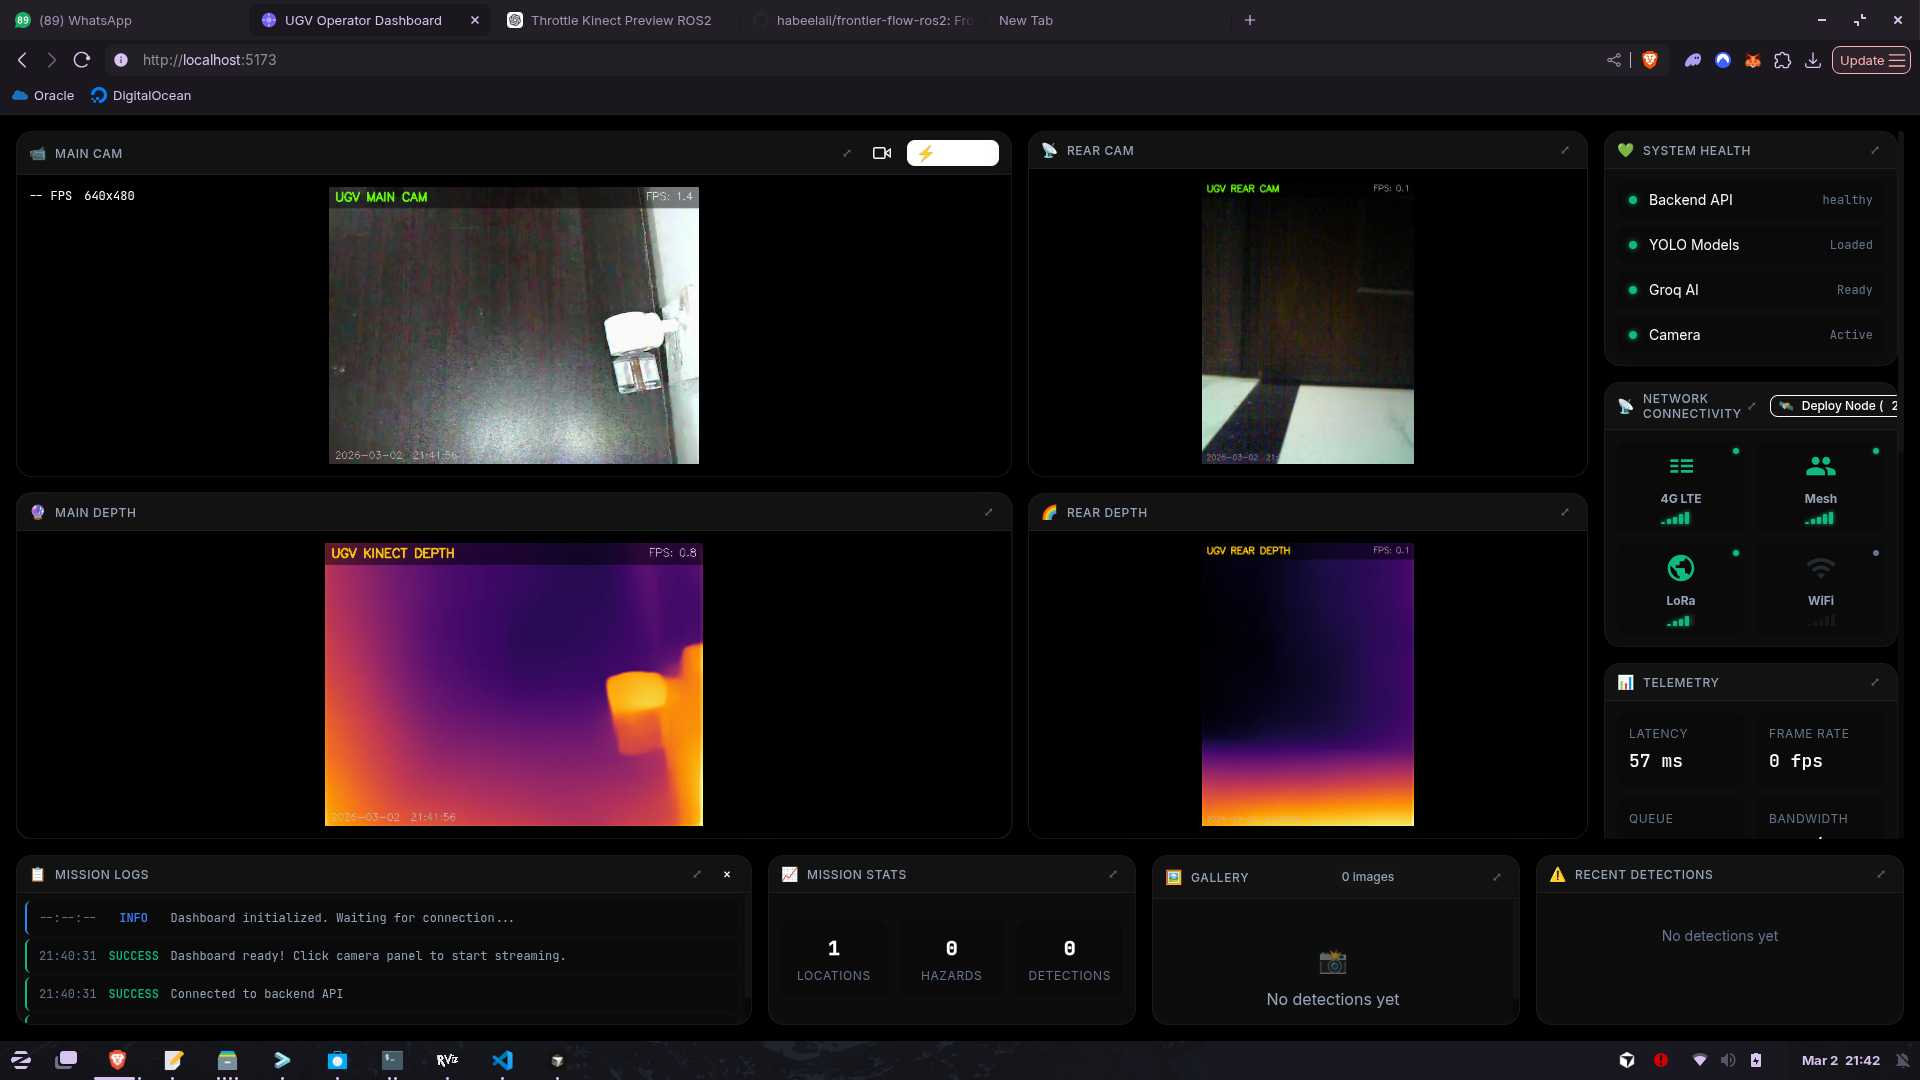
\includegraphics[width=0.5\textwidth]{figures/dashboard.png}
\end{center}
\end{frame}

% --- Comparison & benchmarks ---
\begin{frame}{Comparison \& Benchmarks}
\begin{itemize}
\item \textbf{Design objectives}: All met (SLAM without odometry, multi-tier comms, operator-side AI, KPIs)
\item \textbf{SLAM}: Drift comparable to Cartographer in literature (e.g.\ 0.21\,m with odometry); our 20--30\,cm in feature-poor without encoders
\item \textbf{Perception}: 70--85\% mAP vs.\ SubT-style 0.77 AP at 1 FPS in harsh conditions
\item \textbf{Exploration}: 19--22\,min full coverage; 260--310\,m$^2$ at 15\,min (Explore-Bench style evaluation)
\end{itemize}
\end{frame}

% --- Conclusions ---
\begin{frame}{Conclusions}
\begin{itemize}
\item Integrated UGV: SLAM + multi-tier communication + AI perception with natural-language reporting
\item Runs on RPi~4 (8\,GB); deployable mesh nodes; AI offloaded to GCS $\Rightarrow$ $\sim$2\,h runtime
\item KPIs met: drift, map resolution, throughput/range, detection accuracy, runtime
\item Fills gap between high-end research systems and practical, resource-constrained single-UGV solutions for indoor disaster reconnaissance
\end{itemize}
\end{frame}

% --- Future work ---
\begin{frame}{Future Work}
\begin{enumerate}
\item \textbf{3D SLAM \& multi-level}: 3D maps for multi-floor, overhangs; stair detection
\item \textbf{Multi-robot \& swarm}: shared mesh and maps; task and frontier allocation; long-lived nodes for follow-on robots
\item \textbf{Harsher scenarios}: smoke, dust, low light; multi-storey and post-disaster sites; thermal/gas sensors; user studies with responders
\end{enumerate}
\end{frame}

\begin{frame}{Thank you}
\begin{center}
\Large Questions?
\end{center}
\end{frame}

\end{document}
